\subsection{任务一}
题目给出的S盒输入大小为$m = 4$bit，输出大小也为$n = m = 4$bit，共$2^4$种不同输入与输出，计算S盒的线性近似表思路为：
先遍历输入掩码$\alpha \in \mathbf{F}_2^4$，再遍历输出掩码$\beta \in \mathbf{F}_2^4$，再遍历所有$2^4$种输入，对于输入$x$，计算
对应线性近似式是否为0
$$
\alpha \cdot x \oplus \beta \cdot S(x)
$$
统计其中为0的个数$N(\alpha,\beta)$，然后在S盒的LAT中赋值$N(\alpha,\beta) - 2^3$。三层遍历结束后即完成S盒的线性近似表的计算。记$\operatorname{par}(v)$为4比特数$v$中1的个数模2，$\land$表示逐位与运算，对应伪代码如算法~\ref{alg:task1-lat}所示。

\begin{algorithm}[H]
    \caption{4比特S盒线性近似表的计算}
    \label{alg:task1-lat}
    \begin{algorithmic}[1]
        \Require 4比特S盒$S[0..15]$
        \Ensure 线性近似表$\mathrm{LAT}[0..15,0..15]$
        \For{$\alpha=0,\ldots,15$}
            \For{$\beta=0,\ldots,15$}
                \State $N\gets 0$
                \For{$x=0,\ldots,15$}
                    \State $p\gets\operatorname{par}(\alpha\land x)$
                    \State $q\gets\operatorname{par}(\beta\land S[x])$
                    \If{$p=q$}
                        \State $N\gets N+1$
                    \EndIf
                \EndFor
                \State $\mathrm{LAT}[\alpha,\beta]\gets N-8$
            \EndFor
        \EndFor
        \State \Return $\mathrm{LAT}$
    \end{algorithmic}
\end{algorithm}

代码运行结果如图~\ref{fig:task1-lat}所示。
\begin{figure}[H]
    \centering
    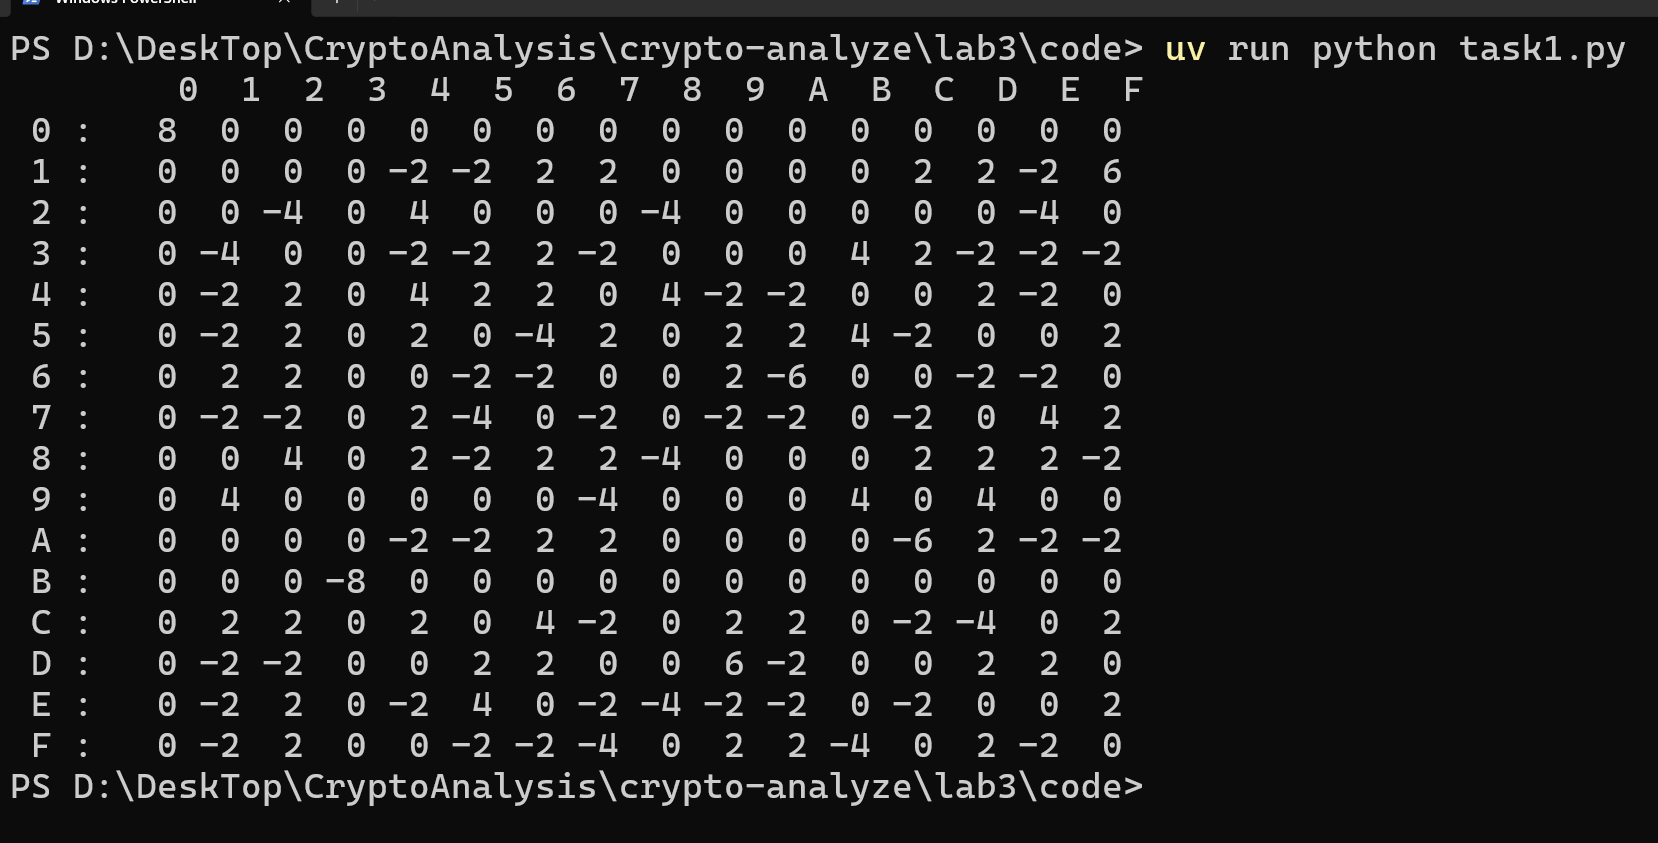
\includegraphics[width=\textwidth]{figures/task1.png}
    \caption{任务一计算得到的S盒线性近似表}
    \label{fig:task1-lat}
\end{figure}
